\chapter{Flight Data}
To begin with the insurance platform, getting data to predict flight delays is the very first step. For accurate prediction, historical data for each flight landing in Germany will be required. One can easily find many open source datasets of historical flight records, but they are limited to United States flight data. As there is no dataset available that fits the project's needs, a new dataset had to be created from scratch that contains all the flight details of Germany for six months. A large number of websites do provide the status of flights but the ones providing historical flight details are few and expensive. For this reason the requirements were defined for the suitable website in the latter sections and the website was selected on the basis of that criteria. Before creating the historical flight dataset though, there is a need to create another smaller dataset. The list of all flights landing in Germany on any given day.

\section{List of all flights landing in Germany}
Getting the list of every flight landing in Germany on a typical day was not an onerous task. The task was divided into two sub-tasks, first of which was getting the complete list of airports in Germany. A quick glance on Flightradar24 website shows the list of 56 airports handling the chartered and commercial flights\footnote{\url{https://www.flightradar24.com/data/airports/germany}}. Airports which handle only chartered flights were not considered. For each airport, a list was available that had records of all the flights landing in that airport on a given day. Each record for these airport was copied into an Excel file, with the most important flight details like destination, origin, airline and flight ID. On completing the copying, the final list consisted of 3000 flights, flying to or within Germany on a given day, from more than 200 airports worldwide.

\section{Plausible Sources for historical flight data}
The next step was to get the historical data of at least 3 months for each flight in the newly created list. Considering that this was going to be a huge dataset that could not be created/curated manually, the requirements for selecting the flightdata's source were defined beforehand as follows:
\begin{enumerate}
    \item The flight data source should have at least 3 months of historical records of flights, especially the actual departure, actual arrival and flight delay.
    \item The flight data source should preferably have a developer friendly API to automate the whole process of retrieving the data.
    \item The API calls limit and subscription costs, if any, for the source should be reasonable.
\end{enumerate}

Based on the above mentioned criteria, the following websites that provide flight records were evaluated.

\subsection{Flightstats}
Flightstats states that it provides the historical data of flights to its registered users. It also provides a REST based API available to its registered users. Registering is not a big issue generally but in case of FlightStats, it is a rather cumbersome ordeal. The user has to give specific domain where the data collected from their website will be used, assure FlightStats there will be no commercial use and give details of what kind of data would be required. On making the request multiple times, my request was rejected. Later a call was made by Flightstats sales team that offered me to provide the complete dataset of historical records of six months of each German flight, as an excel file. The happiness of receiving the complete and clean data was shortlived though as the company asked \EUR{2000} for the dataset, a discounted price for students, which was otherwise double of what was quoted. Hence Flightstats was not considered anymore.

\subsection{Flightaware}
Flightaware on the other hand had an easy registration process. Their developer API is well documented and provides REST API support. Even the developer key is provided free of cost on request. The limitation of the free account is that historical records of only 14 days are provided. A special tier, available for \EUR{20} per month, does provide access to last 5 months of historical flight records\footnote{\url{https://flightaware.com/commercial/premium/}}. But on further research, it was noted that  the historical data was just for display. Their API, FlightXML 3 doesn't provide any particular support for making REST requests for historical data of a flight\footnote{\url{[https://flightaware.com/commercial/flightxml/pricing_class.rvt}}. Hence Flightaware too was not selected.

\subsection{Flightradar24}
Flightradar24 is one of the most famous sites on internet with mobile apps available for iPhone and Android. Flightradar24 does have historical data of 6 months for their Gold tier customers at just \$4 per month. Unfortunately, Flightradar24 provides no API to retrieve that data automatically. Being out of options, this site was selected on the basis of providing maximum amount of data and providing the cheapest premium option.

\section{Getting data}
Not having an API for getting flight history was an obstacle in collecting data. The only option remaining to retrieve the data was scraping it from their webpage. Web Scraping is a technique in which the desired data is extracted from a webpage's HTML output. Having the flight records of last 6 month of flight records as a webpage meant the whole dataset could be created by scraping the data.
\\Even though some websites specifically consider web scraping illegal\cite{Hirschey2014SymbioticScraping}, flightradar24 only rejects web-scraping of data if that data is to be used commercially. The proposed website being a master thesis project, doesn't fit under the commercial category, neither provides anyone actual commercial service. 

\subsection{Web Scraping}
As mentioned earlier, web scraping is basically looking into the source code of a webpage and saving the data desired. Using the previously created list of flights landing in Germany on any given day, a list of URLs was created with the help of this URL template \url{https://www.flightradar24.com/data/flights/<flight_id>/}, where flight\_id was replaced with the Flight ID of each of the flights. 
Once the list of all the web-URLs to be scraped was completed, the actual scraping was started. The language of choice for scraping is Python, as the website was also to be created using Python. The commonly used python library, Scrapy, was used for scraping. Each of the URLs in the list prepared earlier was passed as argument to Scrapy HTTP request function and the desired data variables from  the HTTP response received were saved.
 

\section{Data Variables}
All the data  retrieved from scraping was saved in a CSV file. The total flight records saved were about 385,000. Once completed, the dataset consisted of the following variables.
\begin{enumerate}
    \item {Departure Airport}
    \\Origin Airport of the flight. This value could be of any airport in the world that has a direct flight to a German airport
    \item {Arrival Airport}
    \\Destination airport of the flight. Always one of the German airports
    \item {Standard Arrival}
    \\The fixed arrival time of a flight time based on the flight schedule, mentioned in the flight plans submitted to the airports
    \item {Actual Arrival}
    \\The actual arrival of the flight, that might be earlier or most probably at or after the standard arrival of the flight
    \item {Standard Departure}
    \\The fixed departure time of a flight time based on the flight schedule, mentioned in the flight plans submitted to the airports.
    \item {Actual Departure}
    \\The actual departure of the flight, that might be earlier or most probably at or after the standard departure of the flight
    \item {Airline}
    \\The company operating the flight.
    \item {Flight ID}
    \\The flight ID is a unique number provided by International Air Transport Organisation to each flight.
    \item {Aircraft}
    \\The type of aircraft for the flight.
    \item {Flight Duration}
    \\Total duration of flight in hours.
\end{enumerate}

\section{Data Cleanup and missing values substitution}
On close inspection of the CSV file with all the stored flight records, it was noted that a lot of columns had some missing values. Hence the next step was to fill in the missing data and correct the incorrect data. One big advantage in cleaning the data was that lots of columns were repetitive in nature. For ex., arrival and destination airports stay same for the flight no matter the date of flight. They were easily fixed. But some of the columns, like flight duration would change everyday. Thus different strategies were created for cleaning missing values for each variable. Microsoft Excel was selected for data cleanup due to its ease of use and data visualisation capabilities.

\subsection{Departure Airport}
Departure Airport stays constant for each Flight ID. In the dataset though, some of the flight IDs had different Departure Airports on few occasions, and few were missing the value. This was rectified for each of the 3000 different flights.

\subsection{Arrival Airport}
The same strategy was applied to Arrival Airport for cleanup as well. But arrival airport had two exceptions as compared to departure airport that had to be considered while cleaning the column.
\begin{enumerate}
    \item Flight diverted
    \\Arrival airport remains constant for each Flight ID except in case the flight is diverted. This was a special case and only happened nine times in the dataset. All these entries were removed from the dataset for the sake of uniformity.
    \item Connecting Flights
    \\There are many indirect flight that connect to German airports. For sake of simplicity, it was decided to keep only flights lading in Germany. For ex, if a flight flew from Delhi to Moscow, and then from Moscow to Frankfurt, only flight that came from Moscow was considered and all details of Delhi-Moscow flight were discarded. 
\end{enumerate} 

\subsection{Standard Arrival}
The Standard Arrival time of a flight does not necessarily stay the same all year long. For ex., it changes on the basis of daylight savings or even as a business decision by an airport or Airline. So
instead of making all values of standard departure same for all historical records of a particular flight, the values for the empty cells were copied from the upper or lower cell in the data belonging to the same flight.

\subsection{Standard Departure}
The same strategy as for Standard Arrival was used for cleaning up Standard Departure too.

\subsection{Actual Arrival}
Arguably the most important variable in the dataset. The actual flight delay will be calculated using this variable. Any row that didn't have this value was removed from the dataset.

\subsection{Actual Departure}
Any values that were missing from actual departure, were assumed to be the same as standard departure.

\subsection{Airline}
Any missing value in the airline column was corrected on the basis of the upper or lower cells in the column. 

\subsection{Flight ID}
This was the basis of the whole web scraping process. Only the flights that had Flight ID were scraped, hence there was no chance of a missing or wrong Flight ID. Still, if there were any repetitions of a Flight ID, the rows were deleted.

\subsection{Aircraft}
For cleaning the missing data in Aircraft, it was assumed that a flight uses same aircraft unless a pattern is noticed where each flight after a certain date uses a different aircraft. Missing values were corrected on the basis of the upper or lower cells in the column.

\subsection{Flight duration}
Another very important variable in the dataset. Any missing value was calculated by subtracting Actual departure from Actual Arrival. All the values were also converted into seconds instead of keeping them in Time format. Any row with flight duration more than 24 hours was deleted.

\section{Adding new variables}
After cleaning the dataset, it was decided to add new variables to the dataset which would hopefully make the predictions better aligned to the project's end goal.

\subsection{Flight delay bins}
The insurance rates provided to the user will be varied based on the flight delay prediction. It was decided that the delays would be calculated based on the following four categories. The goal of the prediction would be to classify the flight delay as one of this class.
\begin{enumerate}
    \item 0 if a flight is less than 15 minutes late
    \item 1 if a flight is 15 or minutes but less than an hour late
    \item 2 if a flight is more than 15 minutes but less than an hour late
    \item 3 if a flight is an hour or more late
\end{enumerate}

\subsection{Weekend}
A simple variable. Using Weekday formula in Excel, a binary variable was created with the value as True if the flight was on weekends and False otherwise.

\subsection{Time Blocks}
Instead of using exact arrival time of the flight, a new variable was created which categorised time to a block of 2 hours duration. For ex., a flight at 8:30 in the morning was classified to block 8 and flight at 15:30 was classified to block 16.

\section{Reducing number of factors}
One problem frequently faced while executing classification algorithms on such a big dataset is the number of categories, or factors, of each variable. The flight records dataset has more than 50 airlines and 80 aircrafts. Algorithms in R like random forest don't accept more than 32 categories. Boosting algorithms like XGBoost on the other hand require indicator columns instead of categorical variables. Converting to indicator columns means that a single column with n categories is converted to n binary columns. Having columns with large number of categories will result in huge number of indicator columns. For these reasons, the categories for some of the columns were reduced.

\subsection{Airline}
There were 67 different airlines in the dataset with Lufthansa being the most popular with 124940 flight records. A large number of airlines though have a comparatively small number of flights. On that basis, it was decided that the airlines with lowest number of flights should be combined in a new airline category called other\_airline.

\begin{figure}[H]
    \centering
    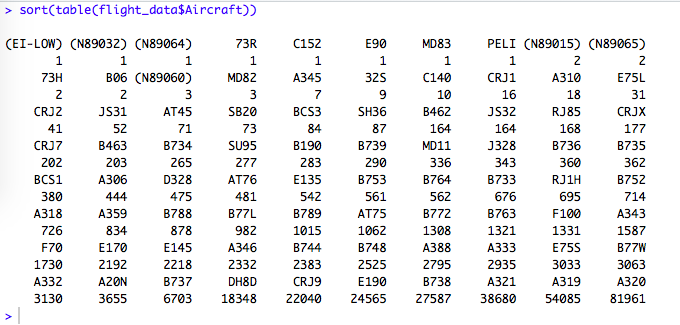
\includegraphics[width=\textwidth]{Figures/Aircraft_orig_levels.png}
    \caption{Reduced categories of Airlines with number of airline}
    \label{fig:airline2}
\end{figure}

\subsection{Aircraft}
There were about 80 different aircrafts in the dataset, with Airbus A320 being the most common choice, having over 81000 flight records. As can be seen in the figure \ref{fig:aircraft1}, there were large number of aircrafts with a insignificant number of flights.

\begin{figure}[H]
    \centering
    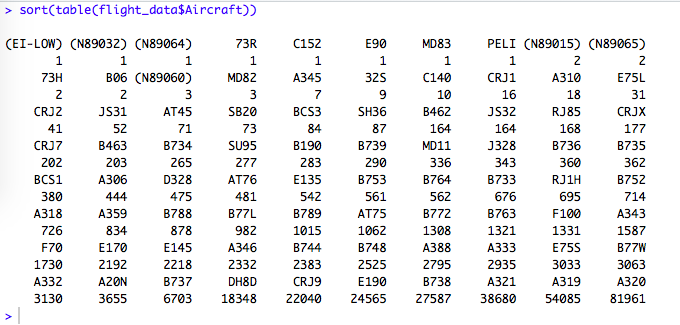
\includegraphics[width=\textwidth]{Figures/Aircraft_orig_levels.png}
    \caption{Original categories of Aircraft with number of flights}
    \label{fig:aircraft1}
\end{figure}

All the aircrafts with the lowest number of flight records were combined to form a new value called other\_aircraft, as seen in figure \ref{fig:aircraft2}.

\begin{figure}[H]
    \centering
    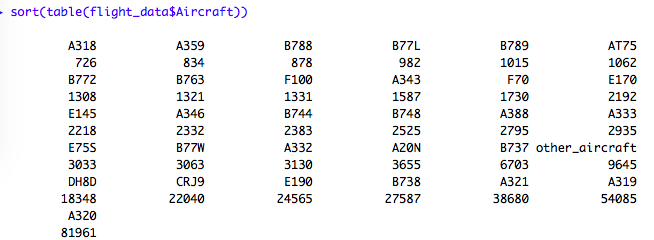
\includegraphics[width=\textwidth]{Figures/Aircraft_reduced_levels.png}
    \caption{Reduced categories of Aircraft with number of flights}
    \label{fig:aircraft2}
\end{figure}

\subsection{Departure Airport}
The departure airport has 287 different departure airports from all over the world. Many of the airports have non-insignificant number of flights so converting a majority of flights to a single category would have been counter-productive. Hence the variable was left as it is 
to. The variable was instead used to create a column with each airport mapped to a country. This is discussed in more detail in the Delay Prediction chapter.

\section{End result - dataset}

After cleaning the data, substituting the missing values, reducing the number of factors and adding new variables to help in prediction, the final summary of the dataset is as seen in figure \ref{fig:summary_flights}:

\begin{figure}[ht]
    \centering
    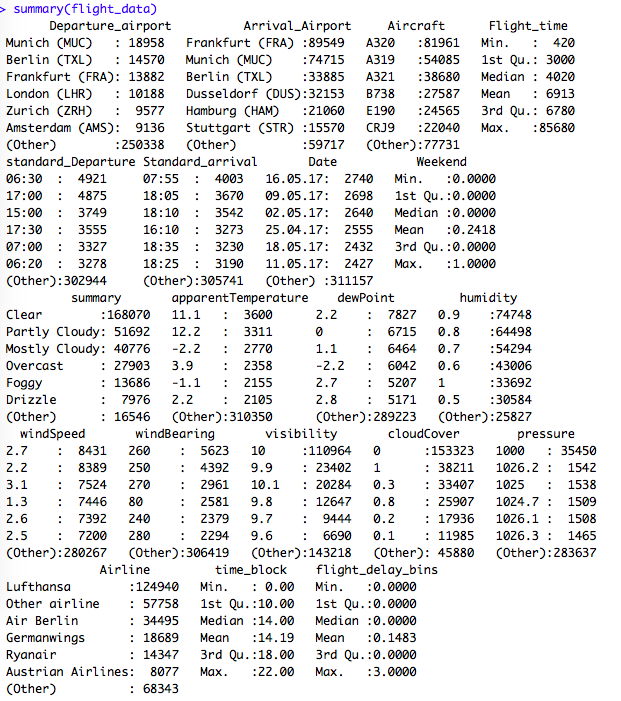
\includegraphics[width=\textwidth]{Figures/summary_flight_data.png}
    \caption{Final summary of our flight dataset}
    \label{fig:summary_flights}
\end{figure}